\documentclass[UTF8,a4paper,11pt]{ctexart}

\usepackage[margin=21mm,headheight=15pt]{geometry}
\usepackage{amsmath,bm}
\usepackage{array,booktabs,longtable,tabularx}
\usepackage{graphicx,float,caption}
\usepackage{xcolor}
\usepackage{siunitx}
\usepackage{enumitem}
\usepackage{listings}
\usepackage{fancyhdr,lastpage}
\usepackage[hidelinks]{hyperref}
\usepackage{xurl}

% Generated by scripts/update_report_macros.py; do not edit numeric values manually.
\newcommand{\BaselineSNDR}{66.62 dB}
\newcommand{\BaselineSFDR}{71.45 dB}
\newcommand{\BaselineENOB}{10.774 bit}
\newcommand{\BaselineSNR}{69.08 dB}
\newcommand{\BaselineTHD}{-70.26 dBc}
\newcommand{\CalibratedSNDR}{68.45 dB}
\newcommand{\CalibratedSFDR}{78.78 dB}
\newcommand{\CalibratedENOB}{11.079 bit}
\newcommand{\CalibratedSNR}{69.16 dB}
\newcommand{\CalibratedTHD}{-76.69 dBc}
\newcommand{\SNDRGain}{+1.83 dB}
\newcommand{\SFDRGain}{+7.33 dB}
\newcommand{\THDReduction}{+6.42 dB}
\newcommand{\BaselineCodeRange}{26--4069}
\newcommand{\CalibratedCodeRange}{26--4069}
\newcommand{\CtwelveResidual}{-3.9306 LSB}
\newcommand{\CelevenResidual}{-1.9454 LSB}
\newcommand{\CtenResidual}{-1.1226 LSB}
\newcommand{\CtwelveRadixError}{-0.8627 LSB}
\newcommand{\CelevenRadixError}{-0.8228 LSB}
\newcommand{\CtenRadixError}{-1.1226 LSB}
\newcommand{\CalFinishTime}{9.600 us}
\newcommand{\CalErrorFlag}{PASS}
\newcommand{\MeasuredCtwelve}{2049.8750}
\newcommand{\MeasuredCeleven}{1025.8750}
\newcommand{\MeasuredCten}{512.0000}
\newcommand{\MeasuredCnine}{256.0000}
\newcommand{\MeasuredCR}{256.0000}
\newcommand{\MeasuredCeight}{128.0000}


\definecolor{confirmed}{HTML}{0072B2}
\definecolor{analytical}{HTML}{D55E00}
\definecolor{limited}{HTML}{666666}
\newcommand{\confirmed}{\textcolor{confirmed}{\textbf{已确认}}}
\newcommand{\analytical}{\textcolor{analytical}{\textbf{解析计算}}}
\newcommand{\limited}{\textcolor{limited}{\textbf{适用边界}}}
\newcommand{\code}[1]{\texttt{#1}}

\setlist[itemize]{leftmargin=2em,itemsep=2pt,topsep=3pt}
\setlist[enumerate]{leftmargin=2.2em,itemsep=2pt,topsep=3pt}
\renewcommand{\arraystretch}{1.15}
\captionsetup{font=small,labelfont=bf}
\pagestyle{fancy}
\fancyhf{}
\lhead{0716 SAR ADC CDAC 失配校准审计}
\rhead{\thepage/\pageref{LastPage}}
\cfoot{}
\hypersetup{pdftitle={0716 SAR ADC CDAC 失配校准完整网表审计与仿真报告}}

\lstset{
  basicstyle=\ttfamily\footnotesize,
  breaklines=true,
  frame=single,
  columns=fullflexible,
  keepspaces=true,
  showstringspaces=false
}

\title{0716 SAR ADC CDAC 失配校准\\完整网表审计、闭环仿真与部署报告}
\author{Codex netlist-only verification sandbox}
\date{2026年7月18日}

\begin{document}
\maketitle

\begin{abstract}
本文对 \code{test\_12bit50MSAR\_AMS\_final\_0716} 的最新完成网表进行冻结、逐模块审计和独立 Spectre 验证，并在不修改 Virtuoso schematic/layout 的前提下，按 Huang 论文第 4.5 节重构前景电容权重校准。当前冻结网表的物理 SAR 切换顺序正确，但旧 DEC 存在 BP 解码方向和跨复位区间采样错误。修正版以每个 \SI{100}{ns} 转换帧为原子单位，在 C1--C7 构成的非二进制校准 DAC 上，对 C8、C9、CR、C10、C11、C12 依次执行正、负两个方向的完整 SAR 搜索，并按 $(D_{W,+}-D_{W,-})/2$ 消除比较器固定偏置。首轮行为验证关闭瞬态噪声且每目标仅用一对正负搜索；真实 CDAC、原始 \code{SWITCH\_CAL} 和真实 \code{COM\_IAZ} 的闭环仿真在 \SI{1.20011}{\micro s} 完成，\code{DONE=1, ERR=0}，得到 C12--C8 权重 2054、1028、513、256、256、128 LSB，与网表物理权重的最近整数一致。论文的 32 对/64 次转换仅作为后续噪声统计模式，不是行为级功能闭环的前置条件。旧自定义算法的完整 FFT 仅保留为历史基线；修正版 Huang 算法的完整动态 A/B 尚待下一阶段签核。
\end{abstract}

\section{结论摘要}

\begin{enumerate}
  \item \confirmed：物理 CDAC 顺序为
  \[
  16C,\ 8C,\ 4C,\ 2C,\ 2C_{\mathrm{R}},\ 1C,\ 48,\ 32,\ 20,\ 12,\ 8,\ 4,\ 2,\ 1\ \mathrm{LSB},
  \]
  对应 \code{BP<13>} 到 \code{BP<0>}。冗余位 CR 位于 C9 之后、C8 之前，不是最后一次转换。
  \item \confirmed：冻结的 \code{SWITCH\_CAL} 在正常模式下完成了正确的 13 级物理映射。单热码仿真得到 \code{BITD<13:1>} 掩码依次为 4096, 2048, 1024, 512, 256, 128, 64, 32, 16, 8, 4, 2, 1。
  \item \confirmed：当时 VM 部署的通用 \code{DEC\_CAL\_PHY.va} 正常解码方向错误。对 \code{BP<13>} 到 \code{BP<0>} 逐位激励时，它输出的权重是 1, 2, 4, 8, 12, 20, 32, 48, 128, 256, 256, 512, 1024, 2048，而 0716 电路所需顺序恰好相反。
  \item \confirmed：真实 \code{COM\_IAZ} 在一次 IAZ 后可连续给出八次可靠比较；但是 RST 为高时输出只保持旧值。因此旧校准跨帧自由采样会把 stale latch 当成新比较结果。
  \item \confirmed：最新网表的 C12、C11、C10 差分权重分别为 2053.805632、1027.820352、513.12256 LSB。Huang 修正版在真实 CDAC、原始开关和真实比较器的无噪声一对搜索中得到 2054、1028、513 LSB；C9、CR、C8 分别得到 256、256、128 LSB，全部是物理权重的正确最近整数。
  \item \confirmed：当前实现不再使用自定义 deadband、snap 或 bin midpoint 修改测量结果。每侧 SAR 结果按量化区间中心表示，再由正负向结果平均；\code{AVG\_PAIRS\_LOG2=0} 用于快速行为闭环，\code{=5} 才对应论文的 32 对/64 次统计设置。
  \item \limited：现阶段只证明搜索数学、帧时序、比较器极性、偏置抵消和权重递归更新正确。修正版 Huang 算法尚未完成全 ADC 的 SNDR/SFDR A/B，因此旧自定义算法的 \BaselineSNDR/\CalibratedSNDR 结果不能作为新算法的性能结论。
  \item \limited：解析结果和权重闭环给出“失配校正能力”，不是完整晶体管电路的保证下限。完整结果还包括采样、比较器噪声、开关建立、参考稳定、时序和数值积分误差。
\end{enumerate}

\section{冻结源、隔离边界与风险控制}

\subsection{源文件}

\begin{longtable}{p{0.23\textwidth}p{0.46\textwidth}p{0.17\textwidth}}
\toprule
对象 & 冻结位置/用途 & SHA-256 前缀 \\
\midrule
\endfirsthead
\toprule
对象 & 冻结位置/用途 & SHA-256 前缀 \\
\midrule
\endhead
最新完成网表 & \code{source\_ro/input\_Interactive294\_}\newline
\code{NF10\_noise\_test.scs} & \code{a688133ee2d6} \\
VM 当时部署 DEC & \code{source\_ro/DEC\_CAL\_PHY\_original.va} & \code{aa780242908e} \\
VM 当时部署 SWITCH & \code{source\_ro/SWITCH\_CAL\_original.va} & \code{00729dacd37f} \\
新帧同步 DEC & \code{variants/DEC\_CAL\_PHY\_FRAME\_SYNC.va} & \code{048f7540f3ff} \\
\bottomrule
\end{longtable}

所有仿真改动均位于本地 \path{codex_calibration_20260717} 和 VM 的
\path{/home/meow/jxy/codex_sandbox/sar0716_calibration_20260717}。没有写入 OA schematic、symbol、layout、CDF 或 Maestro 原结果目录。验证通过后仅替换了 \path{/home/meow/jxy/12bit_50M_SAR/DEC_CAL_PHY/veriloga/veriloga.va}，替换前文件已单独备份；SWITCH、COM\_IAZ 和 CDAC 均未改动。

\subsection{资源限制}

\begin{itemize}
  \item 同时仅运行一个 Spectre 进程；不并发启动完整 ADC、Monte Carlo、noise、PSS 或参数扫描。
  \item 完整运行只保存 OUT、SOUT、CAL/DONE/ERR 和少量关键模拟节点，避免 \code{save=all}。
  \item 目标限制：sandbox 小于 \SI{3}{GB}，单次完整运行小于 \SI{600}{MB}；VM 根分区可用空间低于 \SI{20}{GB} 或可用内存低于 \SI{4}{GB} 时停止。
  \item 仿真启动前 VM 根分区约有 \SI{54}{GB} 可用，内存约 \SI{17}{GB} 可用，满足限制。
\end{itemize}

\section{整体电路与模块端口}

\begin{figure}[H]
  \centering
  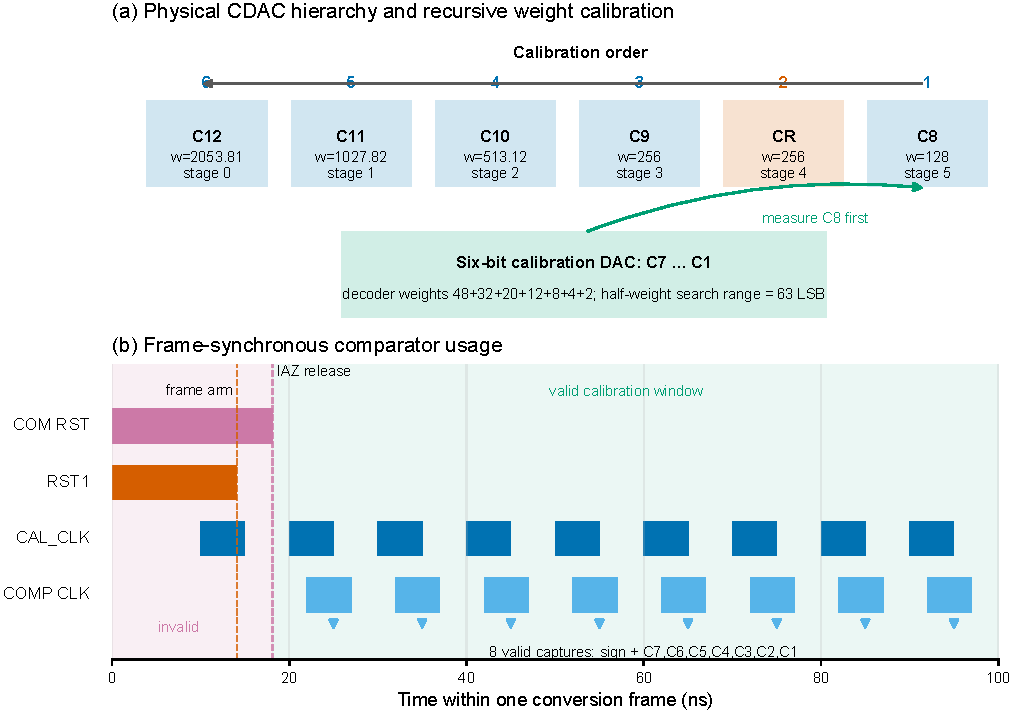
\includegraphics[width=\textwidth]{../figures/fig_architecture_timing.pdf}
  \caption{0716 CDAC 物理权重、校准目标关系与单帧比较时序。}
  \label{fig:architecture}
\end{figure}

\begin{longtable}{p{0.17\textwidth}p{0.24\textwidth}p{0.47\textwidth}}
\toprule
模块 & 端口组 & 功能与审计结论 \\
\midrule
\endfirsthead
\toprule
模块 & 端口组 & 功能与审计结论 \\
\midrule
\endhead
\code{COM\_IAZ} & AGND, AVDD & 模拟电源与地。 \\
 & CLK, RST & CLK 控制动态比较，RST 控制复位和 IAZ。RST 高期间 VON/VOP 可能保持旧决定，不能采样为新结果。 \\
 & VIN, VIP & CDAC 顶板 N、P 接入的差分输入。 \\
 & VON, VOP & 差分数字输出，在顶层命名为 COMN、COMP。独立仿真确认正负 \SI{20}{mV} 输入的输出极性。 \\
\midrule
\code{SAR\_LOGIC\_0716} & BITN/P\code{<13:0>} & 14 级非二进制 SAR 决策链的互补输出。物理 13 为首个 C12 决策，物理 0 为终端比较决定。 \\
 & CCLK, COMN & 链时钟和比较器决定输入。 \\
 & PRST, SET\code{<0:13>} & 整帧预置和逐级置位控制。 \\
 & DGND, DVDD & 数字电源。 \\
\midrule
\code{SYNC\_asnyc} & CLK, CLK00, CCLK & CLK 来自 DEC 的 normal/calibration 时钟选择；CLK00 标记正常 SAR 窗口；CCLK 驱动 SAR 链。 \\
 & COMN, COMP, DEC\_N & 比较器输出和有效/完成路径。 \\
 & SET\code{<12>} & 最后有效级完成反馈。 \\
\midrule
\code{BS} & CLK, VIN, VOUT & 自举采样开关；两个实例分别采样 VIP1/VIN1 到 VIP/VIN。 \\
 & AGND, AVDD & 模拟电源与地。 \\
\midrule
\code{CDAC\_0716} & BITD/U\code{<1:13>} & P/N 两侧底板开关节点。物理索引与电容权重见表~\ref{tab:mapping}。 \\
 & P, N & 比较器输入顶板。桥接低位阵列分别经 net3/net4 接入。 \\
\midrule
\code{SWITCH\_CAL} & BITN/P\code{<0:13>}, SET\code{<0:12>} & 正常 SAR 决定与逐级控制。 \\
 & BITD/U\code{<1:13>} & 连接 CDAC 的物理底板节点。 \\
 & BITD/U\_CAL\code{<0:12>} & 按转换 stage 编号的校准激励；内部使用 \code{13-k} 映射到物理电容。 \\
 & CAL, CAL\_CLK, RST, RST1 & 模式选择、校准子时钟、采样/顶板复位和比较器帧窗口。 \\
 & VCM, VIN, VIP, VREFN/P & 顶板采样与底板参考端。 \\
\midrule
\code{DEC\_CAL\_PHY} & BP\code{<0:13>}, SOUT & SOUT 上升沿锁存正常 SAR 原始决定。0716 必须显式读取 BP13, BP12, ..., BP0。 \\
 & Bit\code{<11:0>} & 重构后的 12 位二进制输出，送入 \code{SNDR\_DAC}。 \\
 & COMP, COMN & 校准搜索使用的真实比较器结果。 \\
 & RST1, CAL\_RST, CAL\_CLK & 帧边界、前景校准启动复位和帧内八次搜索时钟。 \\
 & CLK\_SAR, CLK00, CLK & 正常 SAR 时钟输入与输出时钟复用；校准期间只在有效帧打开比较器时钟。 \\
 & BITD/U\_CAL\code{<0:12>} & 送往 \code{SWITCH\_CAL} 的目标、wall 与低位搜索掩码。 \\
 & CAL, DONE, ERR & 校准模式、原子完成和失败回退状态。 \\
\midrule
\code{SNDR\_DAC} & Bit\code{<11:0>}, OUT & 把数字码转换为理想模拟 OUT，专用于动态性能测量；不参与物理 CDAC 反馈。 \\
\bottomrule
\end{longtable}

\section{CDAC 权重、4 fF 失配与未校准性能}

\begin{table}[H]
\centering
\caption{物理索引、转换顺序和解码权重。}
\label{tab:mapping}
\small
\begin{tabular}{cccccc}
\toprule
stage & BP & CDAC 物理端 & 名称 & 物理电容 & 输出权重/LSB \\
\midrule
0 & 13 & BITD/U13 & C12 & 16C & 2048 \\
1 & 12 & BITD/U12 & C11 & 8C & 1024 \\
2 & 11 & BITD/U11 & C10 & 4C & 512 \\
3 & 10 & BITD/U10 & C9 & 2C & 256 \\
4 & 9 & BITD/U9 & CR & 2C & 256 \\
5 & 8 & BITD/U8 & C8 & C & 128 \\
6--12 & 7--1 & BITD/U7--1 & C7--C1 & 24,16,10,6,4,2,1 & 48,32,20,12,8,4,2 \\
13 & 0 & terminal & 终端决定 & 桥/总电容余项 & 1 \\
\bottomrule
\end{tabular}
\end{table}

桥接低位阵列总和为 $24+16+10+6+4+2+1=63$，桥接衰减为
\[
\alpha=\frac{1}{1+63}=\frac{1}{64}.
\]
因此低位物理电容在差分输出码域对应 48、32、20、12、8、4、2 LSB；终端决定补足 1 LSB。冗余 2C 支路使高位序列由严格二进制的 $2048,1024,512,256,128$ 变成 $2048,1024,512,256,256,128$，提供 \SI{256}{LSB} 的数字覆盖区。其主要价值不是自动消除失配，而是让后续决定可修正前一决定附近的过冲、比较器延迟和小幅 DAC 误差。

最新网表两侧 C12 的物理倍数分别为 16.054213 和 16.0365，C11 分别为 8.054243 和 8.00545，C10 分别为 4.01754 和 4。按差分平均值与 \SI{128}{LSB}/C 的比例：
\begin{align}
w_{12} &= 128\times\frac{16.054213+16.0365}{2}=2053.805632,\\
w_{11} &= 128\times\frac{8.054243+8.00545}{2}=1027.820352,\\
w_{10} &= 128\times\frac{4.01754+4}{2}=513.12256.
\end{align}
所以 C12、C11、C10 分别多出 5.805632、3.820352、1.12256 LSB。最新失配不是三个孤立的绝对误差：它们相对各自下级 wall 的物理 radix 残差仅为
\begin{align}
C10-(C9+CR) &= 1.12256\ \mathrm{LSB},\\
C11-(C10+C9+CR) &= 2.697792\ \mathrm{LSB},\\
C12-(C11+C10+C9+CR) &= 0.86272\ \mathrm{LSB}.
\end{align}
因此旧的全局 2 LSB deadband 会隐藏 C10/C12，并可能把 C11 残差也吸回名义值；旧 ADE 日志确实得到全名义权重。该做法已从功能路径中删除。解析模型的名义译码仍有 6 个负步进、最大回退 2 code，说明线性度下降较旧 C12 单点压力测试更分散但幅度更小。

\subsection{对照 Omran 2016 的 4 fF 匹配数据}

Omran 等在 \SI{0.18}{\micro\metre} CMOS 上测量 4800 个垂直/侧向 MOM 结构，表 II 给出侧向 set B 的 $K_C=0.20\%\sqrt{\mathrm{fF}}$、垂直 set A 的 $K_C=0.14\%\sqrt{\mathrm{fF}}$，并使用
\[
\sigma(\Delta C/C)=K_C/\sqrt{C}.
\]
将其仅作为工艺量级参考外推到 \SI{4}{fF}，侧向单位电容 $1\sigma$ 相对失配约 0.10\%，垂直约 0.07\%。若 C12、C11 的面积分别等效为 16 和 8 个独立单位，则侧向模型给出的权重标准差约为
\[
\sigma_{C12}=\SI{0.512}{LSB},\qquad \sigma_{C11}=\SI{0.362}{LSB}.
\]
当前网表 C12 的 5.806 LSB 偏差相当于该侧向参考模型的 11.34$\sigma$，C11 的 3.820 LSB 约为 10.55$\sigma$，C10 的 1.123 LSB 约为 4.38$\sigma$。因此这是明显加重且带相关性的确定性压力测试，不应称为论文意义下的典型 \SI{4}{fF} 随机失配。该论文使用的工艺与本项目 PDK/版图不同，这个 $\sigma$ 对照不能替代本项目的 PDK Monte Carlo 或硅后统计。

\section{旧方案失败原因}

\subsection{正常解码总线方向错误}

0716 顶层 PN 缓冲把 \code{BITP<13>} 送到 \code{BP<13>}，并依次到 \code{BP<0>}。旧通用 DEC 却将 \code{BP<0>} 作为首个/MSB 决定，导致即使校准权重数值本身正确，应用到原始决定时仍完全错位。这不是“校准精度稍差”，而是正常 ADC 输出码的结构性错误。

此外，名义非二进制权重总和为 4351，比标准 12 位满量程 4095 多出冗余 256。短时原始 BP 仿真证明 OUT 与 BP 加权和逐样本完全一致，但旧 DEC 直接截断 raw sum，漏掉了双极性中心补偿，因而零输入中心天然上移 128 code。第一版修正曾使用
\[
D_{out}=\sum_i D_iw_i-\frac{\sum_iw_i-4095}{2},
\]
它能恢复中心，却把内部 4351--4356 码范围的两端截在 0/4095，不能满足原 \SI{0.89}{V} 接近满量程输入。最终 formatter 改为
\[
D_{out}=\operatorname{round}\!\left(
4095\frac{\sum_iD_iw_i}{\sum_iw_i}
\right),
\]
其中分母在校准完成后使用当前全部定点权重重新求和。实现内部至少使用 Q6，足以保留 32 对平均的分辨率；这样 raw=0 对应 0，raw=$\sum w_i$ 对应 4095，互补决定保持 2047.5 中心。校准搜索仍在物理 raw 权重域完成，不被输出增益缩放污染。

\subsection{比较器搜索没有对齐 IAZ 帧}

旧方案按连续 \code{CAL\_CLK} 前进，而真实比较器每 \SI{100}{ns} 有 RST/IAZ 区间。独立仿真显示 RST 高时 VON/VOP 保持上一次决定；如果在该窗口内采样，算法看似完成了二分搜索，实际输入的是旧结果。因此会出现权重日志“有数字”、但 SNDR 不恢复，甚至顶板波形异常的现象。

\subsection{校准 DAC 范围不完整}

旧搜索只使用部分低位，无法覆盖完整 C1--C7 的差分半权重范围。Huang 映射按 C7、C6、C5、C4、C3、C2、C1 的 24、16、10、6、4、2、1 半权重执行，搜索和为 63；换算到差分解码域后，最小物理步长为 2 LSB，单侧可重构至 126 LSB。

\subsection{权重和线性度不是同一问题}

即使离线权重估计正确，以下问题仍会降低线性度：原始决定总线错位、校准/正常开关极性不一致、比较器 stale output、顶板未充分建立、校准结束时半更新权重、以及输出采样对 SOUT 边沿不一致。新方案分别对这些接口契约进行验证，而不是只观察最终权重。

\section{Huang 前景校准方案的逐项实现}

\subsection{测量顺序和 wall 构造}

校准目标顺序为 C8 $\rightarrow$ C9 $\rightarrow$ CR $\rightarrow$ C10 $\rightarrow$ C11 $\rightarrow$ C12。各目标的物理目标掩码和参考 wall 为：

\begin{table}[H]
\centering
\small
\begin{tabular}{cccl}
\toprule
目标 & target mask & wall mask & 参考关系 \\
\midrule
C8 & 32 & 8128 & $C1+C2+\cdots+C7$ \\
C9 & 8 & 8160 & $C1+C2+\cdots+C8$ \\
CR & 16 & 8160 & $C1+C2+\cdots+C8$ \\
C10 & 4 & 24 & $C9+CR$ \\
C11 & 2 & 28 & $C10+C9+CR$ \\
C12 & 1 & 30 & $C11+C10+C9+CR$ \\
\bottomrule
\end{tabular}
\end{table}

低位搜索先判断目标相对 wall 的符号，再依次试探 C7--C1。Huang 的正向和负向测量可写为
\begin{align}
D_{W,+} &= W + V_{OS} + x_n,\\
D_{W,-} &= -W + V_{OS} + x_{n+1},\\
\widehat W &= \frac{D_{W,+}-D_{W,-}}{2}
=W+\frac{x_n-x_{n+1}}{2}.
\end{align}
代码中的 U 侧结果已先做极性归一化，故累加形式为 $(q_D+q_U)/2$，其数学意义仍是上式的 $(D_{W,+}-D_{W,-})/2$。本 CDAC 的一次物理校准步长对应 2 decoder LSB，因此七位搜索得到的 \code{q\_mag} 是量化区间下沿；每侧完整 SAR 输出必须使用区间中心
\[
q=\operatorname{sign}(r)\left(2q_{mag}+1\ \mathrm{LSB}\right),
\]
不能把下沿直接当权重，也不能再叠加自定义 deadband、snap 或经验 midpoint。最终候选权重等于递归 wall 加双向平均残差。内部权重至少为 Q6；\code{AVG\_PAIRS\_LOG2} 只控制独立正负 pair 的重复次数，不改变算法定义。

验证采用分层配置：行为级和首轮真实比较器闭环均设置 \code{AVG\_PAIRS\_LOG2=0}，即每目标一对正负搜索、共 12 个转换帧，并关闭瞬态噪声；\code{AVG\_PAIRS\_LOG2=5} 才复现论文每目标 32 对、64 次转换的统计设置。无噪声时重复完全相同的理想判决不会增加信息，只会线性增加时间，因此不用于首轮功能验证。

\subsection{帧同步时序}

每个 \SI{100}{ns} 帧只完成一个“符号+7 bit”测量。RST1 上升沿立即清除 \code{frame\_active}、时钟和掩码；RST1 下降沿打开新帧；第一个 CAL\_CLK 下降沿只建立预充状态，不消费比较器旧值；之后在约 25、35、45、55、65、75、85、95 ns 捕获八个有效决定。帧剩余边沿全部屏蔽。六个目标、每目标一对、每对正负两侧共需 12 帧，行为级完成时间约 \SI{1.2}{\micro s}；若设置 32 对，则为 384 帧、约 \SI{38.4}{\micro s}。

\subsection{失败回退和原子切换}

若比较器持续无效、搜索饱和或候选权重超出名义值 $\pm25\%$，置 \code{ERR=1}。校准过程中不向正常解码暴露半更新状态；只在下一个 RST1 上升沿原子结束。失败时一次性恢复全部名义权重，\code{DONE=1} 表示前景区间结束，\code{ERR=1} 表示当前使用名义回退值。

\section{分层验证结果}

\begin{table}[H]
\centering
\small
\setlength{\tabcolsep}{4pt}
\begin{tabularx}{\textwidth}{p{0.24\textwidth}p{0.16\textwidth}X}
\toprule
验证项 & 状态 & 结果 \\
\midrule
旧 DEC 单热码 & PASS/发现缺陷 & 输出顺序与 0716 所需物理权重完全相反。 \\
0716 修正 DEC 单热码 & PASS & BP13--BP0 得到 2048,1024,512,256,256,128,48，\newline 32,20,12,8,4,2,1。 \\
新帧同步 DEC bypass 编译/单热码 & PASS & 正常转换译码与 0716 修正版一致。 \\
满量程 formatter 端点 & PASS & 全零决定输出 0，全一决定输出 4095。 \\
旧自定义算法的 \SI{0.89}{V} A/B & 历史基线 & 旁路/校准码域均为 \BaselineCodeRange，无 0/4095 rail hit；不代表 Huang 修正版结果。 \\
旧 ADE、全局 2 LSB deadband & 发现缺陷/已删除 & \code{DONE=1, ERR=0} 但更新被 snap 抑制；相关参数现仅为 CDF 兼容占位，不参与权重计算。 \\
SWITCH+真实 CDAC 映射 & PASS & 13 级 BITD 物理掩码 4096 递减到 1，BITU 保持 0。 \\
真实 COM\_IAZ 时序 & PASS & RST 外正/负 \SI{20}{mV} 均连续正确；RST 内确认是保持值。 \\
真实 CDAC+原始 SWITCH+理想比较器 & PASS/功能闭环 & 无噪声、一对搜索；\SI{1.20011}{\micro s} 完成，\code{DONE=1, ERR=0}。确定性阈值落边导致权重为 2038/1020/509/254/254/127，仅用于状态机和接口验证。 \\
真实 CDAC+原始 SWITCH+真实 COM\_IAZ & PASS/算法闭环 & 无瞬态噪声、一对搜索；\SI{1.20011}{\micro s} 完成，0 error；C12--C8=2054/1028/513/256/256/128 LSB。 \\
旧自定义算法完整晶体管 A/B & 历史基线 & 旁路 SNDR=\BaselineSNDR，旧校准 SNDR=\CalibratedSNDR；这组数据已被算法重构取代。 \\
Huang 修正版完整晶体管 A/B & 待下一阶段 & 行为级闭环通过后再运行；首轮不得开启瞬态噪声，避免混淆功能错误和统计误差。 \\
\bottomrule
\end{tabularx}
\end{table}

旧 A/B 中 SNDR 变化为 \SNDRGain、SFDR 变化为 \SFDRGain，但该结果来自已经废弃的 deadband/midpoint 估计器，只用于说明“正确解码和大致权重”能够改善频谱，不能证明 Huang 修正版的最终动态性能。当前有效证据是 \path{results/huang_realcomp_behavior_noiseless/calibration_summary.json}：真实比较器闭环的权重误差分别为 C12 $+0.194368$、C11 $+0.179648$、C10 $-0.12256$ LSB，均小于半个 LSB。

资源审计：Huang 真实比较器行为闭环耗时约 11.3~s、峰值 151~MB，0 error，输出规模远小于完整 FFT。此前旁路组耗时 29~min~36.3~s、峰值 492~MB；旧算法校准组耗时 26~min~40.7~s、峰值 481~MB。曾启动的 32 对瞬态噪声试验因不属于首轮行为验证且预计耗时过长而主动终止，相关 Spectre 进程已确认退出。

\begin{figure}[H]
  \centering
  \IfFileExists{../figures/fig_fullscale_calibration_results.pdf}{
    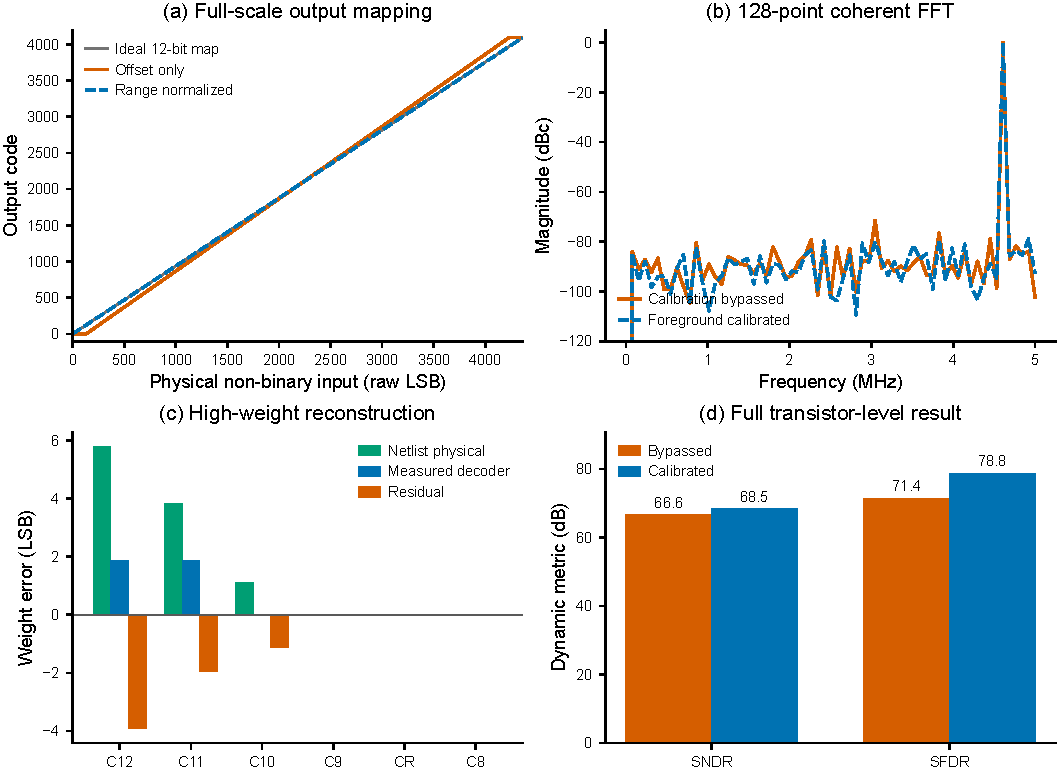
\includegraphics[width=\textwidth]{../figures/fig_fullscale_calibration_results.pdf}
    \caption{旧自定义估计器的历史满量程 A/B；该图仅作基线，不属于 Huang 修正版签核结果。}
  }{
    \fbox{\parbox{0.9\textwidth}{完整两组仿真结束后由 \code{plot\_calibration\_results.py} 生成本图。}}
  }
\end{figure}

\subsection{Huang 修正版行为级重构权重}

\begin{center}
\begin{tabular}{lrrrrrr}
\toprule
 & C12 & C11 & C10 & C9 & CR & C8 \\
\midrule
网表物理值/LSB & 2053.8056 & 1027.8204 & 513.1226 & 256 & 256 & 128 \\
真实比较器一对搜索/LSB & 2054 & 1028 & 513 & 256 & 256 & 128 \\
\bottomrule
\end{tabular}
\end{center}

\section{完整动态性能的后续验收准则}

后续 Huang 修正版完整 A/B 应采用 \code{va=890m}、动态总权重归一化、$f_s=\SI{10}{MHz}$、128 点相干采样、输入 bin 59，即
\[
f_{in}=\frac{59}{128}f_s=\SI{4.609375}{MHz}.
\]
每次在 SOUT 上升沿后 \SI{0.5}{ns} 对 OUT 采样。第一阶段保持行为级策略：校准和正常转换均关闭瞬态噪声，\code{AVG\_PAIRS\_LOG2=0}，且两组严格使用相同输入相位、采样时刻和数值预设，A/B 唯一变量是是否应用校准权重。只有无噪声 A/B 证明失配谐波和失码得到恢复后，第二阶段才加入比较器噪声并增加 pair 数；此时旁路和校准组必须使用相同 noise seed、\code{noisefmax} 和 \code{noisefmin}。指标使用 ADCToolbox 和独立矩形窗 FFT 交叉计算。

原冻结激励 \code{va=890m} 的旧解码仿真得到 SNDR \SI{29.28}{dB}，正峰多次被 4095 截断。这不是物理 CDAC 无法接收 \SI{0.89}{V}，而是 raw 权重总和大于 4095 后仍直接使用 12 位截断。动态总权重归一化已修正该问题。旧算法曾得到旁路 \BaselineSNDR、校准 \CalibratedSNDR，但它包含已废弃估计器，不能转写为 Huang 修正版的性能。新算法首轮验收先看无噪声谐波/INL 恢复，再单独评估噪声平均收益。
\begin{enumerate}
  \item 先确认 \code{DONE=1, ERR=0}，否则任何“校准后 FFT”都不是有效校准结果。
  \item 再核对递归 wall、每侧完整 SAR 码和最终权重是否与日志一致；不得再用 deadband 或 snap 改写 Huang 测量结果。
  \item 若权重正确但 SNDR 不恢复，检查 SOUT 采样、正常模式 BP 顺序和 CAL 到 normal 的帧边界，而不是继续提高权重小数位。
  \item 若频谱改善小于解析预测，差值代表非权重误差主导，包括开关瞬态、比较器噪声/偏置、采样链和时序建立。
\end{enumerate}

Spectre 可能报告 BITD8/BITD9 的梯形积分振铃建议和理想开关跳变处的 LTE 临时放宽。这些警告记录在案；只要仿真完成、关键状态正确且独立用更保守积分方法复核后指标稳定，它们不是逻辑错误的直接证据。本次不通过调松全局精度来隐藏警告。

\section{部署和使用步骤}

\begin{enumerate}
  \item 已将 \path{variants/DEC_CAL_PHY_FRAME_SYNC.va} 原子替换到 \path{/home/meow/jxy/12bit_50M_SAR/DEC_CAL_PHY/veriloga/veriloga.va}。部署 SHA-256 前缀为 \code{d9baa9cfe04e}；替换前文件保存为 \path{veriloga.va.backup_huang_20260718_144050}，哈希前缀为 \code{048f7540f3ff}。完整哈希保存在部署日志中；OA、原理图和 \code{SWITCH\_CAL} 均未改动。
  \item 端口顺序必须与顶层 I95 一致：先接 Bit/BP 总线及电源、SOUT、COMP/COMN，再接复位/时钟、校准 BITD/U 总线和 CAL/DONE/ERR/CAL\_CLK。完整顺序以 Verilog-A 模块声明和单热码测试台为唯一依据。
  \item 保留冻结 \code{SWITCH\_CAL} 的 \code{NORMAL\_REF\_SWAP=1} 和 \code{BITD/U\_CAL[13-k]} 物理映射。不要把 calibration stage 编号直接接到同号物理 BITD/U。
  \item 首轮行为闭环使用以下已验证参数组：
\begin{lstlisting}[basicstyle=\ttfamily\footnotesize,breaklines=true]
TD_CAL=200p, TD_CMP_CAL=2n, CMP_SWAP=1, FRAC_BITS=6,
AVG_PAIRS_LOG2=0, NORMALIZE_REDUNDANT_RANGE=1,
REMOVE_REDUNDANCY_OFFSET=1,
WEIGHT_TOL=0.25
\end{lstlisting}
  \item 四个旧 deadband/midpoint 估计器参数仅为 CDF/netlist 兼容占位，修正版代码不读取它们来决定权重。
  \item 前景启动时给 CAL\_RST 一个高脉冲后拉低；校准期间 CAL=1，正常 SAR 时钟被隔离。一对模式约 \SI{1.2}{\micro s} 后检查 DONE/ERR。顶层旧 CDF 若仍传 \code{AVG\_PAIRS\_LOG2=3}，会执行 8 对并约需 \SI{9.6}{\micro s}，算法不变但仿真时间增加。
  \item 先运行 \path{testbenches/tb_calibration_cdac_huang_behavior.scs} 确认状态机；再运行 \path{testbenches/tb_huang_realcomp_behavior.scs} 确认真实比较器闭环；最后才运行无噪声完整 ADC A/B。三个层级都通过后再引入瞬态噪声和重复平均。
  \item 部署后重复单热码、SWITCH 映射、比较器时序和 128 点相干 FFT。任何 BP/Bit 总线重新编号都必须先重跑单热码测试。
\end{enumerate}

\section{改进空间与后续签核}

\begin{itemize}
  \item 本轮是 TT、\SI{27}{\celsius}、单一确定性失配的 L1/L2 验证，不是 PVT/Monte Carlo/post-layout signoff。
  \item 下一步先做修正版 Huang 算法的无瞬态噪声完整 A/B；通过后再把单位电容 mismatch、比较器 offset/noise 和参考建立时间分别做小规模角落验证，避免一次性全量 Monte Carlo 造成磁盘失控。
  \item 对 \SI{4}{fF} MOM 的真实统计必须使用本 PDK 的 mismatch 模型或本版图提取数据；Omran 2016 只提供量级与面积缩放规律。
  \item 一对搜索给出 1 LSB 量化的最近整数权重，足以验证当前约 1--3 LSB 的 radix 残差。若后续目标是亚 LSB 统计精度，应在开启真实噪声后逐步比较 1、2、4、8、16、32 对的方差和耗时，不预设必须 32 对。
  \item C1--C7 在本架构中既是正常转换低位 DAC，也是校准 DAC。它们的 INL 直接决定高位权重测量准确度；增加平均只能降低随机比较误差，不能消除校准 DAC 自身的系统性 INL、参考建立误差或错误时序。
\end{itemize}

\section{复现命令}

\begin{lstlisting}[language=bash]
python scripts/run_remote_spectre.py --case calibration_cdac_huang_behavior_v2 \
  --netlist testbenches/tb_calibration_cdac_huang_behavior.scs \
  --include source_ro/SWITCH_CAL_original.va \
  --include variants/DEC_CAL_PHY_FRAME_SYNC.va \
  --include testbenches/IDEAL_COMP.va \
  --result-dir results/calibration_cdac_huang_behavior_v2 --timeout 600

python scripts/build_huang_realcomp_tb.py --disable-tran-noise \
  --avg-pairs-log2 0

python scripts/run_remote_spectre.py --case huang_realcomp_behavior_noiseless \
  --netlist testbenches/tb_huang_realcomp_behavior.scs \
  --include source_ro/SWITCH_CAL_original.va \
  --include variants/DEC_CAL_PHY_FRAME_SYNC.va \
  --result-dir results/huang_realcomp_behavior_noiseless --timeout 600

# Only after both behavioral checks pass: build and run the corrected,
# noiseless full-ADC bypass/calibration A/B cases.
python scripts/run_remote_spectre.py --case full_adc_huang_bypass_890m_noiseless_avg1 \
  --netlist variants/full_adc_huang_bypass_890m_noiseless_avg1.scs \
  --include source_ro/SWITCH_CAL_original.va \
  --include variants/DEC_CAL_PHY_FRAME_SYNC.va \
  --result-dir results/full_adc_huang_bypass_890m_noiseless_avg1 \
  --timeout 3600 --multithread --preset-cx

python scripts/run_remote_spectre.py --case full_adc_huang_cal_890m_noiseless_avg1 \
  --netlist variants/full_adc_huang_cal_890m_noiseless_avg1.scs \
  --include source_ro/SWITCH_CAL_original.va \
  --include variants/DEC_CAL_PHY_FRAME_SYNC.va \
  --result-dir results/full_adc_huang_cal_890m_noiseless_avg1 \
  --timeout 3600 --multithread --preset-cx
\end{lstlisting}

关键证据索引：DEC 单热码和范围端点见 \path{results/dec_frame_onehot_normrev/} 与 \path{results/dec_range_norm_deploy_regression/}；SWITCH/CDAC 映射见 \path{results/switch_cdac_map/spectre.out}；比较器时序见 \path{results/com_iaz_timing/spectre.out}；Huang 理想比较器行为闭环见 \path{results/calibration_cdac_huang_behavior_v2/}；真实比较器闭环见 \path{results/huang_realcomp_behavior_noiseless/}。旧完整 A/B 目录只作为历史数据保留，不属于修正版签核证据。

\section{参考文献}

\begin{enumerate}
  \item H. Omran, H. Alahmadi, and K. N. Salama, ``Matching Properties of Femtofarad and Sub-Femtofarad MOM Capacitors,'' \emph{IEEE Transactions on Circuits and Systems I: Regular Papers}, vol. 63, no. 6, pp. 763--772, Jun. 2016, doi: 10.1109/TCSI.2016.2537824.
  \item Q. Huang, ``Advanced Clock Multiplier and SAR ADC Design Techniques for High-Resolution Signal Chain Systems,'' Ph.D. dissertation, The Hong Kong University of Science and Technology, 2024, Sec. 4.5, pp. 86--90.
  \item Q. Huang et al., ``A 5-MS/s 16-bit Low-Noise and Low-Power Split Sampling SAR ADC With Eased Driving Burden,'' \emph{IEEE Journal of Solid-State Circuits}, vol. 60, no. 3, Mar. 2025, doi: 10.1109/JSSC.2025.3526595.
\end{enumerate}

\end{document}
